\chapter{Ingestion: From PDFs to a Searchable Index}
\label{ch:ingestion}

Ingestion is the offline half of the system. It turns two textbook PDFs into 3,608 citable passages, each stored with its 768-number embedding in a Qdrant collection. Everything about a later citation --- the book, the section, the printed page --- is decided here. A mistake in this chapter's code would make citations wrong while every later stage appears to work, which is why the code is unusually defensive.

\section{Overview}

\begin{center}
\begin{tabularx}{\textwidth}{@{}>{\raggedright\arraybackslash}p{2.6cm}>{\raggedright\arraybackslash}p{3.3cm}>{\raggedright\arraybackslash}p{3.9cm}L@{}}
\toprule
\textbf{Step} & \textbf{Module} & \textbf{Input $\rightarrow$ output} & \textbf{Main job}\\
\midrule
1. Registry & \code{ingest/corpus.py} & --- $\rightarrow$ \code{BookSpec} & Declare which books, which edition, which licence.\\
2. Download & \code{ingest/download.py} & URL $\rightarrow$ PDF + manifest & Fetch idempotently, resumably, atomically; record checksums.\\
3. Parse & \code{ingest/parse.py} & PDF $\rightarrow$ \code{PageText} & Text per page with chapter, section and printed page; remove noise.\\
4. Chunk & \code{ingest/chunk.py} & \code{PageText} $\rightarrow$ \code{Chunk} & Sentence-aligned passages of at most 512 tokens with overlap.\\
5. Embed and store & \code{llm/provider.py}, \code{store/collection.py} & \code{Chunk} $\rightarrow$ Qdrant point & Vectors, deterministic ids, citation payloads.\\
Orchestration & \code{ingest/pipeline.py} & PDFs $\rightarrow$ index + run report & Resumable batches; provenance.\\
\bottomrule
\end{tabularx}
\end{center}

Two commands run it: \code{vidyarag download} and \code{vidyarag ingest}. Neither needs an API key.

\begin{measured}[a full rebuild from the PDFs, 13 September 2026]
\code{vidyarag ingest --recreate} into a scratch collection took 1,944 seconds (32 minutes) on the development machine's CPU and produced exactly the shipped index's counts:

\begin{center}
\begin{tabular}{@{}lrrrr@{}}
\toprule
\textbf{Book} & \textbf{PDF pages} & \textbf{Pages parsed} & \textbf{Chunks} & \textbf{PDF size}\\
\midrule
Biology & 1,480 & 1,273 (86\%) & 1,765 & 279\,MB\\
Anatomy and Physiology & 1,420 & 1,289 (91\%) & 1,843 & 135\,MB\\
\midrule
Total & 2,900 & 2,562 & 3,608 & 415\,MB\\
\bottomrule
\end{tabular}
\end{center}

The same page and chunk counts appear in \code{docs/EVALUATION.md}. The working index occupies 34.9\,MB on disk.
\end{measured}

\section{Step 1: the corpus registry}
\label{sec:corpus}

\code{corpus.py} declares the corpus once, as immutable data. Its docstring calls it \enquote{the single source of truth for which books VidyaRAG indexes and under what licence}, and adds that if \code{ATTRIBUTION.md} ever disagrees, \enquote{this file is what actually ran} \ev{src/vidyarag/ingest/corpus.py:1-5}.

\begin{lstlisting}[language=Python]
@dataclass(frozen=True, slots=True)
class BookSpec:
    slug: str            # used in file names, chunk ids, manifest keys
    title: str
    edition: str
    published: str
    source_url: str      # rendered in citations and attribution
    pdf_url: str
    book_uuid: str
    print_isbn_13: str
    license_name: str = "CC BY 4.0"
    license_url: str = "https://creativecommons.org/licenses/by/4.0/"
    publisher: str = "OpenStax, Rice University"
\end{lstlisting}
\vspace{-4pt}{\raggedleft\ev{src/vidyarag/ingest/corpus.py:36-76} (abridged)\par}

\begin{center}
\begin{tabularx}{\textwidth}{@{}>{\raggedright\arraybackslash}p{2.8cm}LL@{}}
\toprule
& \textbf{\code{BIOLOGY}} & \textbf{\code{ANATOMY_AND_PHYSIOLOGY}}\\
\midrule
Slug & \code{biology} & \code{anatomy-and-physiology}\\
Edition, published & 1st, 2016-10-21 & 1st, 2013-04-25\\
Print ISBN-13 & 978-1-938168-09-3 & 978-1-938168-13-0\\
Licence & CC BY 4.0 & CC BY 4.0\\
\bottomrule
\end{tabularx}
\end{center}

\paragraph{Why exactly these two books.} The docstring records that the licence was verified per title \emph{and per edition} against OpenStax's content API, because OpenStax relicensed much of its catalogue at the second edition: \emph{Biology 2e}, \emph{Anatomy and Physiology 2e}, \emph{Microbiology} and \emph{Concepts of Biology} are CC BY-NC-SA 4.0. Only the first editions remain CC BY 4.0, \enquote{which makes them the complete usable biology corpus rather than a preference among many} \ev{src/vidyarag/ingest/corpus.py:16-26}. A second reason is recorded beside the \code{CORPUS} tuple: the books are complementary, overlapping only in Biology's animal-systems unit, and that \enquote{shallow seam} makes genuine cross-book multi-hop questions possible without the redundancy that would make context precision ambiguous \ev{src/vidyarag/ingest/corpus.py:101-109}.

The git history shows this was a correction, not the original plan: the first corpus commit after scaffolding is titled \enquote{fix(attribution): correct false CC BY claim; switch corpus to CC BY editions} \ev{git 85d4f8b}.

\paragraph{Where the licence goes.} \code{license_name} and \code{source_url} are copied onto every stored passage, so attribution \enquote{survives retrieval instead of being bolted on at the UI layer}.

\section{Step 2: download}
\label{sec:download}

The module promises three properties \ev{src/vidyarag/ingest/download.py:7-15}:

\begin{description}[style=nextline]
  \item[Idempotent.] If the PDF is already on disk, the network is never touched; the file is hashed and its pages counted.
  \item[Resumable.] An interrupted transfer continues with an HTTP \code{Range} request instead of starting over.
  \item[Atomic.] Bytes are written to \code{<name>.pdf.part} and renamed only after the full body has been read, so a crash can never leave a truncated file that looks complete.
\end{description}

\begin{lstlisting}[language=Python]
for _ in range(2):
    resume_from = part.stat().st_size if part.exists() else 0
    headers = {"Range": f"bytes={resume_from}-"} if resume_from else {}
    with httpx.stream("GET", spec.pdf_url, headers=headers,
                      follow_redirects=True, timeout=_TIMEOUT) as response:
        # 416 means the .part is already >= the asset: stale, not partial.
        if response.status_code == httpx.codes.REQUESTED_RANGE_NOT_SATISFIABLE:
            part.unlink(missing_ok=True)
            continue
        # A 200 in reply to a Range request means the server ignored it.
        if resume_from and response.status_code == httpx.codes.OK:
            resume_from = 0
        response.raise_for_status()
        with part.open("ab" if resume_from else "wb") as handle:
            for block in response.iter_bytes(_STREAM_CHUNK_BYTES):
                handle.write(block)
        return
raise RuntimeError(f"Could not download {spec.slug}: ...")
\end{lstlisting}
\vspace{-4pt}{\raggedleft\ev{src/vidyarag/ingest/download.py:115-149} (progress reporting removed)\par}

\begin{background}[HTTP range requests]
A client can ask for part of a resource with a header such as \code{Range: bytes=1048576-}. A server that supports it replies \code{206 Partial Content}. A server that does not support it may ignore the header and send the whole file with \code{200 OK}. If the requested start lies beyond the end of the file, the reply is \code{416 Range Not Satisfiable}.
\end{background}

The loop handles all three replies: 206 appends, 200 overwrites (because the server is sending the whole body), and 416 deletes the stale partial file and retries once without a \code{Range} header, which cannot produce another 416. Each case has a test with a mocked HTTP server \ev{tests/test\_download.py}.

\paragraph{The manifest.} After fetching, \code{download_corpus} writes \code{data/raw/manifest.json} with a \code{DownloadRecord} per book: slug, title, edition, file name, both URLs, SHA-256, size, page count, licence, UUID, ISBN and a timestamp \ev{src/vidyarag/ingest/download.py:49-79}. Opening the PDF to count pages \enquote{doubles as an integrity check}: a checksum proves the bytes are unchanged, but only opening the document proves they are a readable PDF rather than an error page \ev{src/vidyarag/ingest/download.py:93-101}.

\paragraph{Checksums are recorded, not verified.} OpenStax publishes no digest to compare against. The stated value of the checksum is detecting drift: \enquote{if a re-download produces a different hash, the upstream asset changed and every downstream number was computed against different text} \ev{src/vidyarag/ingest/download.py:17-21}.

\begin{inferred}[limits of that drift detection]
\code{download_corpus} writes a fresh manifest without reading the previous one \ev{src/vidyarag/ingest/download.py:217-221}, so drift is only detected if a person compares the new manifest with an old copy. Separately, \code{downloaded_at} is set to the current time even when nothing was downloaded \ev{src/vidyarag/ingest/download.py:195}, so after a re-run it records when the file was last \emph{verified}, not when it was fetched.
\end{inferred}

\section{Step 3: parsing}
\label{sec:parse}

The parser's job is stated precisely in its docstring: not \enquote{get the text out} but \enquote{get the text out \emph{and} know where it came from} \ev{src/vidyarag/ingest/parse.py:3-6}. Figure~\ref{fig:parse-flow} shows what happens to each page.

\begin{figure}[htbp]
\centering
\scalebox{1}{%
\begin{tikzpicture}[
  font=\sffamily\footnotesize,
  node distance=4mm and 8mm,
  proc/.style={draw, rounded corners=2pt, fill=blue!6, align=center, text width=52mm, minimum height=9mm},
  dec/.style={draw, diamond, aspect=2.6, fill=orange!12, align=center, inner sep=1pt, text width=26mm},
  drop/.style={draw, rounded corners=6pt, fill=red!8, align=center, text width=26mm, minimum height=7mm},
  arr/.style={-Stealth, thick}
]
\node[proc] (toc) {\code{load_outline}: read \code{doc.get_toc()},\\drop entries without a page, sort by (page, level)};
\node[proc, below=of toc] (map) {\code{build_structure_map}: page $\rightarrow$ (chapter, section);\\excluded ranges left out};
\node[dec, below=of map] (inmap) {page in map?};
\node[drop, right=of inmap] (d1) {skip page\\(front matter, index, answer key)};
\node[proc, below=of inmap] (blocks) {\code{_ordered_blocks}: text blocks only; drop header and footer bands; order two columns};
\node[proc, below=of blocks] (clean) {\code{clean_text}: rejoin hyphenated breaks, trim, collapse blank lines};
\node[proc, below=of clean] (strip) {\code{strip_end_matter}: cut at REVIEW / CRITICAL THINKING / ... QUESTIONS};
\node[dec, below=of strip] (empty) {empty, or\\$\ge$4 options a.--d.?};
\node[drop, right=of empty] (d2) {skip page};
\node[proc, below=of empty] (emit) {yield \code{PageText}(book, PDF page, printed page from running head, chapter, section, text)};
\draw[arr] (toc) -- (map);
\draw[arr] (map) -- (inmap);
\draw[arr] (inmap) -- node[above, font=\scriptsize]{no} (d1);
\draw[arr] (inmap) -- node[left, font=\scriptsize]{yes} (blocks);
\draw[arr] (blocks) -- (clean);
\draw[arr] (clean) -- (strip);
\draw[arr] (strip) -- (empty);
\draw[arr] (empty) -- node[above, font=\scriptsize]{yes} (d2);
\draw[arr] (empty) -- node[left, font=\scriptsize]{no} (emit);
\end{tikzpicture}}
\caption{What \code{extract_pages} does with each page \ev{src/vidyarag/ingest/parse.py:310-352}.}
\label{fig:parse-flow}
\end{figure}

\subsection{Structure from the outline, not from fonts}

OpenStax PDFs carry an outline (the bookmarks panel of a PDF viewer), which gives real (level, title, page) entries. The alternative, guessing headings from font size, \enquote{misfires on pull quotes, figure captions, and section headers that happen to wrap, and it fails silently} \ev{src/vidyarag/ingest/parse.py:8-11}. If a PDF has no outline, \code{extract_pages} raises \code{ValueError} rather than producing citations it cannot justify \ev{src/vidyarag/ingest/parse.py:326-331}.

\code{load_outline} does two defensive things. It collapses non-breaking spaces, because outline titles arrive as \lstinline~"Chapter\xa01.\xa0The Study of Life"~ and would otherwise break string comparisons and render as boxes. And it sorts entries by page, because \emph{Biology} ends with a stray \enquote{Blank Page} entry pointing at page 6; left in document order, that single entry \enquote{swallows the whole book into one bogus range} \ev{src/vidyarag/ingest/parse.py:144-168}.

\code{build_structure_map} then assigns every page to the most recent outline entry at or before it. The shallowest outline level counts as a chapter and resets the section; any deeper entry sets the section.

\begin{example}[building the page map from a small outline --- illustrative page numbers]
{\small
\begin{tabularx}{\linewidth}{@{}c>{\raggedright\arraybackslash}p{5.0cm}rL@{}}
\toprule
\textbf{Level} & \textbf{Title} & \textbf{Page} & \textbf{Pages it owns}\\
\midrule
1 & Preface & 5 & 5--12: \emph{excluded, absent from the map}\\
1 & Chapter 1. The Study of Life & 13 & 13: (Chapter 1, no section)\\
2 & 1.1. The Science of Biology & 14 & 14--26: (Chapter 1, 1.1)\\
2 & 1.2. Themes and Concepts of Biology & 27 & 27--44: (Chapter 1, 1.2)\\
1 & Chapter 2. The Chemical Foundation of Life & 45 & 45 onwards: (Chapter 2, no section)\\
\bottomrule
\end{tabularx}\par}
A page's range ends one page before the next entry starts. Because the map is keyed by page, every page belongs to exactly one (chapter, section) pair.
\end{example}

\paragraph{Exclusions.} An outline title matching \code{preface}, \code{index}, \code{solution(s)}, \code{answer key}, \code{references}, \code{appendix}, \code{about openstax}, \code{table of contents}, \code{contents} or \code{blank page} removes its pages \ev{src/vidyarag/ingest/parse.py:55-59}. The comment singles out \enquote{Solutions}, OpenStax's answer key: about 35 pages of bare answers \enquote{phrased in the same vocabulary as the questions, so it competes for exactly the queries the book should answer and satisfies none of them.} Exclusion \enquote{inherits downwards but never sideways}: an excluded chapter removes its sections, but an excluded section does not remove its siblings. Both rules have tests \ev{tests/test\_parse.py}.

The word \enquote{Glossary} is \emph{not} excluded. End-of-chapter key terms and summaries sit under a trailing Glossary heading in the outline and are kept on purpose, because \enquote{summaries are condensed explanation and key terms are definitions, both of which answer real questions} \ev{src/vidyarag/ingest/parse.py:67-75}.

\subsection{Reading a page in the right order}

\begin{figure}[htbp]
\centering
\begin{tikzpicture}[font=\sffamily\scriptsize, blk/.style={draw, fill=blue!8, minimum width=24mm, align=center}]
\draw[thick, fill=white] (0,0) rectangle (6,8.4);
\fill[red!12] (0,7.9) rectangle (6,8.4);
\fill[red!12] (0,0) rectangle (6,0.5);
\node at (3,8.15) {188 \quad Chapter 6 \textbar{} Metabolism};
\node at (3,0.25) {footer text};
\node[blk, minimum height=8mm] (l1) at (1.55,7.05) {L1};
\node[blk, minimum height=14mm] (l2) at (1.55,5.6) {L2};
\node[blk, minimum height=18mm] (l3) at (1.55,3.6) {L3};
\node[blk, minimum height=12mm] (l4) at (1.55,1.6) {L4};
\node[blk, minimum height=18mm] (r1) at (4.45,6.5) {R1};
\node[blk, minimum height=16mm] (r2) at (4.45,4.3) {R2};
\node[blk, minimum height=16mm] (r3) at (4.45,2.1) {R3};
\draw[dashed, gray] (3,0.6) -- (3,7.8);
\draw[-Stealth, orange!80!black, thick] (l1) -- (l2);
\draw[-Stealth, orange!80!black, thick] (l2) -- (l3);
\draw[-Stealth, orange!80!black, thick] (l3) -- (l4);
\draw[-Stealth, orange!80!black, thick] (l4.east) to[out=0, in=180] (r1.west);
\draw[-Stealth, orange!80!black, thick] (r1) -- (r2);
\draw[-Stealth, orange!80!black, thick] (r2) -- (r3);
\node[anchor=west, align=left] at (6.3,8.15) {header band: blocks ending in the top 6\% are dropped\\(the printed page number is read from here first)};
\node[anchor=west, align=left] at (6.3,0.25) {footer band: blocks starting below 94\% are dropped};
\node[anchor=west, align=left] at (6.3,4.2) {gutter: a vertical gap no block crosses,\\at least 4\% of the page width wide,\\its centre within 18\% of the page centre;\\the widest such gap wins};
\node[anchor=west, align=left] at (6.3,2.3) {reading order: left column top to bottom,\\then right column top to bottom};
\end{tikzpicture}
\caption{How \code{_ordered_blocks} and \code{_column_split} turn a page's text blocks into reading order \ev{src/vidyarag/ingest/parse.py:222-277}. Block positions are illustrative.}
\label{fig:page-layout}
\end{figure}

PyMuPDF returns a page's text as blocks with coordinates. \code{_ordered_blocks} keeps text blocks (type 0), drops blocks lying entirely in the top 6\% or bottom 6\% of the page (running heads and footers), and then asks \code{_column_split} whether the page has two columns. That function sorts the blocks' horizontal extents and sweeps from left to right, tracking the rightmost edge reached so far; every uncovered horizontal gap is a candidate gutter. A candidate counts only if it is at least 4\% of the page width and its centre lies within 18\% of the page's centre, and the widest qualifying gap wins. With a gutter, the left column is read top to bottom, then the right. Without one, blocks are read top to bottom, then left to right.

The docstring ranks the three layout fixes by the damage each prevents: running heads would otherwise \enquote{embed as noise on every single chunk}; naive extraction of two-column pages \enquote{produces text that looks plausible and is actually shredded}; and hyphenated line breaks would split words into tokens that \enquote{never match a query} \ev{src/vidyarag/ingest/parse.py:13-22}.

\subsection{Cleaning and removing question pages}

\begin{lstlisting}[language=Python]
_HYPHEN_BREAK = re.compile(r"([A-Za-z])-\n([a-z])")
_MULTI_NEWLINE = re.compile(r"\n{3,}")
_TRAILING_SPACE = re.compile(r"[ \t]+\n")

def clean_text(raw: str) -> str:
    text = _HYPHEN_BREAK.sub(r"\1\2", raw)
    text = _TRAILING_SPACE.sub("\n", text)
    text = _MULTI_NEWLINE.sub("\n\n", text)
    return text.strip()
\end{lstlisting}
\vspace{-4pt}{\raggedleft\ev{src/vidyarag/ingest/parse.py:88-92, 280-290}\par}

\begin{finding}[a comment that describes the opposite of its regex]
The comment above \code{_HYPHEN_BREAK} says: \enquote{"photosyn-\textbackslash nthesis" -> "photosynthesis", but never "well-\textbackslash nknown" -> "wellknown" for a genuinely hyphenated compound: only rejoin when the tail is lowercase} \ev{src/vidyarag/ingest/parse.py:88-90}. But \code{known} begins with a lowercase letter, so the pattern \lstinline~([A-Za-z])-\n([a-z])~ \emph{does} turn \lstinline~well-\nknown~ into \code{wellknown}. What the code actually preserves is a hyphen followed by an uppercase letter, and that is what the test checks (\enquote{Uppercase tail means a real hyphenated term, not a line break}) \ev{tests/test\_parse.py:120-124}. Lowercase hyphenated compounds that happen to break at a line end lose their hyphen. The effect on retrieval is likely small, but the comment should not be quoted as behaviour.
\end{finding}

End-of-chapter question sets have no outline entry of their own, so they are recognised from the text. \code{strip_end_matter} cuts a page at the first of five uppercase headings (\code{REVIEW QUESTIONS}, \code{CRITICAL THINKING QUESTIONS}, \code{ART CONNECTION QUESTIONS}, \code{VISUAL CONNECTION QUESTIONS}, \code{INTERACTIVE LINK QUESTIONS}). Question blocks that continue onto later pages have no heading, so \code{is_question_page} drops any page with four or more multiple-choice option markers of the form \code{a.}~\ldots~\code{d.} followed by a space \ev{src/vidyarag/ingest/parse.py:76-84, 293-307}. \code{docs/EVALUATION.md} records that removing question sets cut about 8.6\% of chunks.

\begin{inferred}[an edge the tests do not cover]
A continuation page of \emph{open-ended} critical-thinking questions has neither a heading nor lettered options, so neither rule removes it, and its text would be chunked as if it were prose.
\end{inferred}

\subsection{Printed page numbers}

A student looks pages up by the number printed on the page, not by the PDF viewer's index. These PDFs declare no page labels (\code{get_label()} returns an empty string), so \code{printed_page_number} reads the number from the running head: at the start on left-hand pages (\enquote{188 Chapter 6 \textbar{} Metabolism}) and at the end on right-hand pages \ev{src/vidyarag/ingest/parse.py:61-65, 355-377}. The docstring gives the concrete stake: PDF page 200 of \emph{Biology} is printed page 188, \enquote{and citing 200 would send a reader to the wrong place.} \code{docs/EVALUATION.md} records offsets of 12 pages for \emph{Biology} and 10 for \emph{Anatomy and Physiology}.

\begin{measured}[printed pages and sections in the working index]
All 3,608 passages carry a printed page number. 61 passages (1.7\%) have a chapter but no section --- text that precedes a chapter's first section.
\end{measured}

\section{Step 4: chunking}
\label{sec:chunking}

\subsection{The rules}

\begin{enumerate}
  \item \textbf{Chunks never cross a section boundary.} Pages are grouped by (book, chapter, section), and each group is chunked independently. A section is the smallest unit the outline guarantees is about one topic, so a chunk's metadata is \enquote{exactly true rather than approximately true} \ev{src/vidyarag/ingest/chunk.py:3-6}.
  \item \textbf{Chunks may cross a page break.} A chunk records the page range it covers and cites the page where it starts.
  \item \textbf{Chunks are built from whole sentences}, greedily, up to 512 tokens.
  \item \textbf{Consecutive chunks overlap} by whole trailing sentences worth up to 64 tokens.
  \item \textbf{Tokens are counted with the embedding model's own tokenizer}, not a generic one.
\end{enumerate}

\paragraph{Why rule 5 matters.} \code{bge-base-en-v1.5} uses BERT WordPiece and truncates hard at 512 tokens, while OpenAI's \code{cl100k_base} tokenizer counts the same English prose about 7\% shorter. Sizing chunks to 512 \code{cl100k_base} tokens would hand the embedder about 548 of its own tokens, and \enquote{the tail of every full-size chunk [would be] silently dropped --- text still shown to the reader and still named in the citation, but contributing nothing to the vector that retrieved it} \ev{src/vidyarag/ingest/chunk.py:12-19}. The 7\% figure is stated in the code, not measured in the repository.

\subsection{Splitting sentences}

\begin{lstlisting}[language=Python]
_SENTENCE_BOUNDARY = re.compile(
    r"(?:(?<=[.!?])|(?<=[.!?][\"'”’)\]]))"  # noqa: RUF001
    r"\s+"
    r"(?=[A-Z“‘(\[\d])"  # noqa: RUF001
)
_ENDS_WITH_ABBREVIATION = re.compile(rf"(?:^|\s)(?:{_ABBREV_ALTERNATION})\.$")
\end{lstlisting}
\vspace{-4pt}{\raggedleft\ev{src/vidyarag/ingest/chunk.py:78-83}\par}

A boundary is whitespace that follows terminal punctuation (optionally closed by a quote or bracket) and precedes something that can start a sentence: a capital letter, an opening quote or bracket, or a digit. Three details are explained in the comments:

\begin{itemize}
  \item The curly quotation marks are deliberate: OpenStax uses typographic quotes, so an ASCII-only class would fail to split after any quoted sentence.
  \item There are two look-behind branches because Python's \code{re} module accepts only fixed-width look-behinds, and an optional closing character would make a single branch variable-width.
  \item Abbreviations (\code{e.g}, \code{i.e}, \code{Fig}, \code{Dr}, \code{approx}, \code{spp} and fourteen others) are handled by gluing a fragment back onto the previous sentence whenever that sentence ends in one, again because a look-behind over alternatives of different lengths is not allowed \ev{src/vidyarag/ingest/chunk.py:37-83, 116-143}.
\end{itemize}

Paragraph breaks are always boundaries.

\begin{inferred}[two consequences of the boundary rule]
A sentence that starts with a lowercase letter --- common in biology, as in \enquote{mRNA carries\ldots} or \enquote{pH falls\ldots} --- is never split from the sentence before it, so the two travel together as one longer unit. And because each page's text is joined with a blank line, a sentence that runs across a page break is split into two pieces at the break. If a chunk boundary falls between those pieces, a chunk can open mid-sentence.
\end{inferred}

\subsection{Packing}

\begin{lstlisting}[language=Python]
for sentence in sentences:
    # a sentence carrying a page marker moves the current page forward
    for marker in _PAGE_MARKER.finditer(sentence):
        page = int(marker.group(1))
    clean = _PAGE_MARKER.sub("", sentence).strip()
    if not clean:
        continue
    cost = count_tokens(clean, embedding_model)

    if cost >= chunk_size:                  # cannot be packed: emit it alone
        if buffer:
            yield emit(buffer, sequence); sequence += 1
            buffer, tokens = [], 0
        yield emit([(clean, cost, page)], sequence); sequence += 1
        continue

    if tokens + cost > chunk_size and buffer:   # full: emit, keep an overlap
        yield emit(buffer, sequence); sequence += 1
        buffer, tokens = _carry_overlap(buffer, chunk_overlap)

    buffer.append((clean, cost, page))
    tokens += cost

if buffer:
    yield emit(buffer, sequence)
\end{lstlisting}
\vspace{-4pt}{\raggedleft\ev{src/vidyarag/ingest/chunk.py:242-271} (reformatted)\par}

Before splitting, each page's text is prefixed with an invisible marker (a NUL character, \code{PAGE:}, the page number, NUL). The markers let the packer know which page each sentence starts on, and are removed from the emitted text \ev{src/vidyarag/ingest/chunk.py:85-86, 150-156}. \code{_carry_overlap} walks backwards through the finished chunk and keeps whole sentences while their total stays within 64 tokens \ev{src/vidyarag/ingest/chunk.py:274-290}.

\begin{figure}[htbp]
\centering
\resizebox{\textwidth}{!}{%
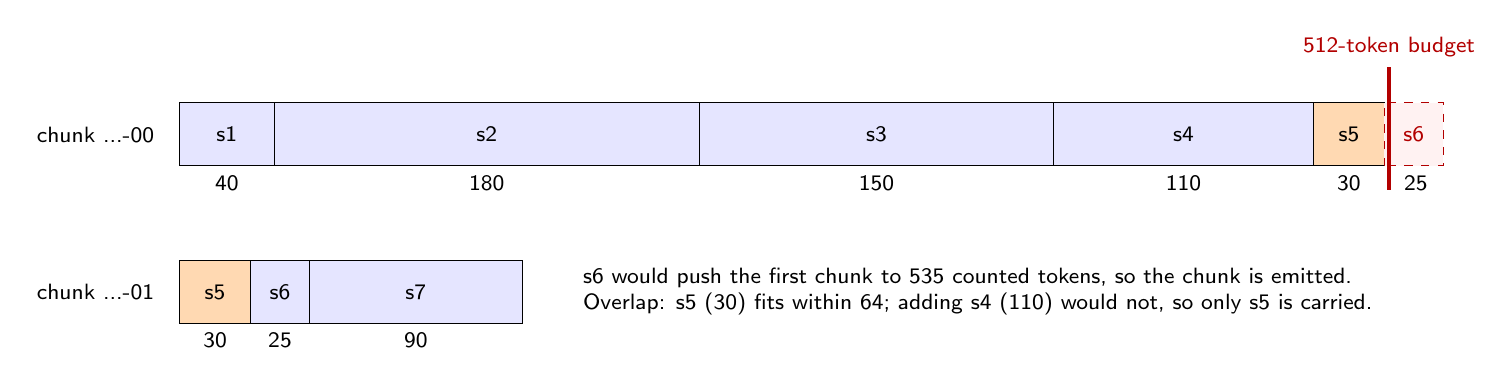
\begin{tikzpicture}[font=\sffamily\footnotesize]
\def\y{1.4}
\draw[fill=blue!10] (0,\y) rectangle (1.2,\y+0.8) node[pos=.5] {s1};
\draw[fill=blue!10] (1.2,\y) rectangle (6.6,\y+0.8) node[pos=.5] {s2};
\draw[fill=blue!10] (6.6,\y) rectangle (11.1,\y+0.8) node[pos=.5] {s3};
\draw[fill=blue!10] (11.1,\y) rectangle (14.4,\y+0.8) node[pos=.5] {s4};
\draw[fill=orange!30] (14.4,\y) rectangle (15.3,\y+0.8) node[pos=.5] {s5};
\draw[dashed, red!70!black, fill=red!5] (15.3,\y) rectangle (16.05,\y+0.8) node[pos=.5] {s6};
\draw[very thick, red!70!black] (15.36,\y-0.3) -- (15.36,\y+1.25) node[above] {512-token budget};
\node[anchor=north] at (0.6,\y) {40}; \node[anchor=north] at (3.9,\y) {180}; \node[anchor=north] at (8.85,\y) {150};
\node[anchor=north] at (12.75,\y) {110}; \node[anchor=north] at (14.85,\y) {30}; \node[anchor=north] at (15.7,\y) {25};
\node[anchor=east] at (-0.2,\y+0.4) {chunk \code{...-00}};
\def\z{-0.6}
\draw[fill=orange!30] (0,\z) rectangle (0.9,\z+0.8) node[pos=.5] {s5};
\draw[fill=blue!10] (0.9,\z) rectangle (1.65,\z+0.8) node[pos=.5] {s6};
\draw[fill=blue!10] (1.65,\z) rectangle (4.35,\z+0.8) node[pos=.5] {s7};
\node[anchor=north] at (0.45,\z) {30}; \node[anchor=north] at (1.275,\z) {25}; \node[anchor=north] at (3.0,\z) {90};
\node[anchor=east] at (-0.2,\z+0.4) {chunk \code{...-01}};
\node[anchor=west, align=left] at (5.0,\z+0.4) {s6 would push the first chunk to 535 counted tokens, so the chunk is emitted.\\ Overlap: s5 (30) fits within 64; adding s4 (110) would not, so only s5 is carried.};
\end{tikzpicture}}
\caption{Greedy packing with overlap, using illustrative sentence token counts. Box widths are proportional to tokens.}
\label{fig:packing}
\end{figure}

\subsection{What a token count really measures}

\begin{measured}[the tokenizer the chunker counts with]
Called directly in the project environment, \code{count_tokens("Hello", "BAAI/bge-base-en-v1.5")} returns 3, because the tokens are \code{[CLS]}, \code{hello}, \code{[SEP]}. An empty string counts as 2. A 1,000-word string counts as exactly 512, because the tokenizer fastembed supplies has truncation enabled at 512 tokens.
\end{measured}

\begin{inferred}[what follows from that measurement]
\begin{enumerate}
  \item \textbf{Chunks come out below the budget.} Every sentence's cost includes two special tokens, but the joined chunk has only one pair. A chunk of $n$ sentences is therefore packed as if it were about $2(n-1)$ tokens longer than it is. This is consistent with the measured maximum chunk size of 487 tokens rather than 512.
  \item \textbf{The overlap is a bound, not a size.} Only whole sentences within 64 counted tokens are carried. If the last sentence of a chunk is longer than that, no overlap is carried at all.
  \item \textbf{Counts cannot exceed 512.} A pathologically long sentence would be counted as 512, emitted alone, and truncated at embedding time. The measured index contains no chunk above 487 tokens, so this has not happened.
\end{enumerate}
\end{inferred}

\subsection{Chunk identity and the \code{Chunk} record}

\begin{lstlisting}[language=Python]
@dataclass(frozen=True, slots=True)
class Chunk:
    chunk_id: str             # f"{slug}-p{start:04d}-{seq:02d}", e.g. "biology-p0388-01"
    book_slug: str
    book_title: str
    chapter: str | None
    section: str | None
    page_start: int           # inclusive PDF page range
    page_end: int
    printed_page: str | None  # printed number at page_start
    text: str
    token_count: int          # recomputed on the joined text

    @property
    def citation(self) -> str:
        where = self.section or self.chapter
        page = self.printed_page or str(self.page_start)
        return f"{self.book_title}, {where}, p.{page}" if where else f"{self.book_title}, p.{page}"
\end{lstlisting}
\vspace{-4pt}{\raggedleft\ev{src/vidyarag/ingest/chunk.py:89-113, 225-240}\par}

The identifier combines the book, the PDF page the chunk starts on, and a sequence number that restarts for each section. A real stored citation looks like \code{Biology, 14.4. DNA Replication in Prokaryotes*, p.376}. The trailing asterisk is part of the section title in the PDF outline.

\begin{inferred}[why chunk ids cannot collide]
A page belongs to exactly one section in the structure map, and the sequence number increases within a section, so no two chunks of one book can share both a start page and a sequence number. The index confirms the absence of collisions: a collision would overwrite a point, yet the 3,608 chunks created produced 3,608 stored points.
\end{inferred}

\begin{measured}[the shape of the 3,608 chunks in the working index]
\begin{center}\small
\begin{tabular}{@{}lr@{\quad}lr@{}}
\toprule
Mean tokens & 428 & Chunks under 120 tokens & 70\\
Median tokens & 455 & Chunks spanning more than one PDF page & 1,990 (55\%)\\
5th / 95th percentile & 206 / 475 & Chunks from Glossary sections & 594 (16.5\%)\\
Minimum / maximum & 44 / 487 & Chunks over 512 tokens & 0\\
\bottomrule
\end{tabular}
\end{center}
\end{measured}

\subsection{Where chunking shows: \enquote{what is tissue?}}

\begin{measured}[a short definitional question, run against the working index]
For \enquote{what is tissue?}, the top dense hit was \emph{Anatomy and Physiology}, 4.1 Types of Tissues, p.136 (cosine score 0.6846), and the reranker kept it first (cross-encoder score 0.4546, against 0.0741 for the second passage). That passage begins in the middle of a sentence and contains no one-line definition. The crisp definitions of \enquote{tissue} are in Glossary passages (\emph{Anatomy and Physiology}, p.172; \emph{Biology}, p.29), which did not reach the five passages given to the model. Adding BGE's recommended query instruction prefix left the top three passages unchanged.
\end{measured}

\code{docs/EVALUATION.md} lists this case under \enquote{What did not work}, and the README's limitations section names short definitional questions as a known weakness that the gold set under-samples.

\section{Step 5: embedding and storage}
\label{sec:store}

\subsection{Embedding}

\begin{lstlisting}[language=Python]
@lru_cache(maxsize=4)
def get_embedder(model_name: str) -> TextEmbedding:
    return TextEmbedding(model_name=model_name)

def embed_texts(texts: list[str], model_name: str, *, batch_size: int = 32) -> list[list[float]]:
    if not texts:
        return []
    embedder = get_embedder(model_name)
    return [vector.tolist() for vector in embedder.embed(texts, batch_size=batch_size)]
\end{lstlisting}
\vspace{-4pt}{\raggedleft\ev{src/vidyarag/llm/provider.py:33-99} (docstrings removed)\par}

The model object is cached per process because building it costs far more than using it; the first call downloads the ONNX weights, which the docstring puts at about 210\,MB and a minute \ev{src/vidyarag/llm/provider.py:37-39}. Ingestion embeds in batches of 64, the same size it uses for upserts \ev{src/vidyarag/ingest/pipeline.py:178-179}.

\subsection{The collection}

\begin{lstlisting}[language=Python]
POINT_NAMESPACE = uuid.UUID("6f3c1e58-9a2b-4d77-9f0e-2c5a8b1d4e63")
DENSE_VECTOR = "dense"

def point_id(chunk_id: str) -> str:
    return str(uuid.uuid5(POINT_NAMESPACE, chunk_id))

client.create_collection(
    collection_name=name,
    vectors_config={DENSE_VECTOR: models.VectorParams(size=dimension,
                                                      distance=models.Distance.COSINE)},
)
\end{lstlisting}
\vspace{-4pt}{\raggedleft\ev{src/vidyarag/store/collection.py:27-43, 87-95}\par}

\begin{description}[style=nextline]
  \item[Deterministic ids make ingestion idempotent.] A \code{uuid5} is a hash of a namespace and a name, so the same chunk id always yields the same point id, on every machine. Writing a chunk again overwrites it. The docstring spells out the alternative: random ids \enquote{would silently double the corpus and quietly wreck every retrieval metric that follows} \ev{src/vidyarag/store/collection.py:3-7}. Tests: \code{test_rewriting_the_same_chunk_does_not_duplicate} and \code{test_second_run_embeds_nothing_and_does_not_duplicate}.
  \item[The vector is named.] Naming it \code{dense} leaves room for a sparse vector beside it. Hybrid search was never built, but renaming the vector later would orphan every stored point, so the name stays \ev{src/vidyarag/store/collection.py:29-38}.
  \item[Dimension mismatches fail early.] Opening an existing collection whose vectors have a different width raises a \code{ValueError} that tells you to re-ingest with \code{--recreate} or choose another collection name, instead of failing \enquote{deep inside an upsert} \ev{src/vidyarag/store/collection.py:75-85}. Test: \code{test_rejects_a_dimension_mismatch}.
  \item[A \code{book_slug} payload index is requested.] It makes per-book filtering cheap on a server or in the cloud. Embedded mode ignores payload indexes and warns; the warning is silenced because the same code must build a correctly indexed collection elsewhere \ev{src/vidyarag/store/collection.py:96-109}.
\end{description}

\paragraph{The payload.} Every point carries 13 fields: \code{chunk_id}, \code{book_slug}, \code{book_title}, \code{chapter}, \code{section}, \code{page_start}, \code{page_end}, \code{printed_page}, \code{citation}, \code{text}, \code{token_count}, \code{license} and \code{source_url} \ev{src/vidyarag/store/collection.py:113-129}. Attribution \enquote{that lives only in a README stops being true the moment a chunk is returned by an API; carrying it on the point means it survives retrieval} \ev{src/vidyarag/store/collection.py:9-11}.

\subsection{Reaching Qdrant}

\code{store/client.py} is \enquote{the only place in the codebase that knows how Qdrant is reached} \ev{src/vidyarag/store/client.py:3-11}. Embedded mode with \code{:memory:} returns \code{QdrantClient(location=":memory:")}; embedded mode with a folder creates the folder and returns \code{QdrantClient(path=...)}; server mode passes the URL; cloud mode passes the URL and API key. \code{describe_target} prints the active target with the key replaced by \code{***}, so logs always show which index a run touched without leaking a secret (test: \code{test_cloud_target_redacts_the_api_key}).

\begin{finding}[a stale size estimate]
\code{store/client.py} explains its 20,000-point advisory threshold by saying the corpus \enquote{is expected to land near 6k chunks} \ev{src/vidyarag/store/client.py:22-25}. The corpus has 3,608. \code{docs/DESIGN.md} repeats the 6,000 estimate.
\end{finding}

\section{The orchestrator}
\label{sec:ingest-orchestrator}

\begin{lstlisting}[language=Python]
ensure_collection(client, collection, embedding_dim, recreate=recreate)
already = set() if recreate else existing_chunk_ids(client, collection)

for spec in books:
    chunks, pages_parsed = chunks_for_book(spec, directory, chunk_size=chunk_size,
                                           chunk_overlap=chunk_overlap,
                                           embedding_model=embedding_model)
    pending = [c for c in chunks if c.chunk_id not in already]
    for batch in _batched(iter(pending), batch_size):
        vectors = embed_texts([c.text for c in batch], embedding_model, batch_size=batch_size)
        points = list(make_points(zip(batch, vectors, strict=True),
                                  license_name=spec.license_name, source_url=spec.source_url))
        embedded += upsert_points(client, collection, points)
    ...
report = IngestReport(...)
report.write(report_path)
\end{lstlisting}
\vspace{-4pt}{\raggedleft\ev{src/vidyarag/ingest/pipeline.py:159-217} (abridged)\par}

\paragraph{Resumability.} Before embedding anything, the orchestrator scrolls the collection in pages of 1,000, reading only the \code{chunk_id} payload field, and skips every chunk already present. It deliberately reads ids rather than trusting a count, because \enquote{a partial run leaves a partial collection, and only the ids say which chunks still need work} \ev{src/vidyarag/store/collection.py:166-190}. Parsing and chunking are always redone; only embedding is skipped. Test: \code{test_resumes_after_a_partial_run}.

\paragraph{The run report.} \code{IngestReport} records start and finish times, duration, collection, embedding model and dimension, chunk size and overlap, total chunks, points in the collection, and per-book pages parsed, chunks created, embedded and skipped \ev{src/vidyarag/ingest/pipeline.py:53-84}. The module docstring calls it \enquote{the provenance record for every number that follows}.

\begin{finding}[the provenance record is written to a fixed place]
\label{sec:finding-ingest-report}
The report path defaults to \code{data/ingest_run.json} under the repository root \emph{whatever index was built} \ev{src/vidyarag/ingest/pipeline.py:45, 80-84}, and \code{vidyarag ingest} does not pass a different path. Building any other index --- another \code{QDRANT_PATH} or another collection --- overwrites the record describing the working index. This happened during this analysis: the scratch rebuild described above replaced the local report, which now names the collection \code{vidyarag_verify_v1}. The working index itself was untouched, and \code{data/} is not tracked by git. The docstring already warns that tests must pass their own path for exactly this reason; the CLI has the same exposure.
\end{finding}

\paragraph{How long ingestion takes.} Three figures exist, and they measure different things. The orchestrator's docstring says embedding 3,600 chunks on CPU \enquote{takes \textasciitilde15 minutes} \ev{src/vidyarag/ingest/pipeline.py:9-12}. \code{docs/EVALUATION.md} reports an index build time of 3,464 seconds (about 58 minutes). The full rebuild measured during this analysis, including parsing, took 1,944 seconds (32 minutes). \NotDet{} which machine and conditions produced the first two figures.

\section{Data structures along the way}

\begin{center}
\begin{tabularx}{\textwidth}{@{}>{\raggedright\arraybackslash}p{2.9cm}>{\raggedright\arraybackslash}p{3.2cm}L@{}}
\toprule
\textbf{Object} & \textbf{Created by} & \textbf{What it adds}\\
\midrule
\code{BookSpec} & \code{corpus.py} & Identity, edition, URLs, licence.\\
\code{DownloadRecord}, \code{Manifest} & \code{download.py} & Checksum, size, page count, timestamp.\\
\code{OutlineEntry} & \code{load_outline} & One bookmark: level, normalised title, 1-based page.\\
\code{PageText} & \code{extract_pages} & Clean text of one page, with chapter, section, PDF page and printed page.\\
\code{Chunk} & \code{chunk_pages} & A sentence-aligned passage with page range, id and token count.\\
\code{PointStruct} & \code{make_points} & Deterministic id, the \code{dense} vector and the 13-field payload.\\
\code{RetrievedChunk} & \code{retrieve_dense} & The payload read back at query time, with a similarity score (Chapter~\ref{ch:retrieval}).\\
\code{IngestReport} & \code{ingest} & Provenance of the whole run.\\
\bottomrule
\end{tabularx}
\end{center}

\section{How ingestion is tested}

The tests run without the real PDFs, without the network and without a Qdrant server. Download tests mock HTTP with respx; storage tests use an in-memory Qdrant. Collected test counts, including parametrised cases, are: \code{test_parse.py} 21, \code{test_chunk.py} 19, \code{test_collection.py} 14, \code{test_download.py} 11, \code{test_pipeline.py} 7 (the ingest orchestrator), \code{test_corpus.py} 7, \code{test_store.py} 7 \tagM. Test names read as specifications, for example \code{test_solutions_is_excluded}, \code{test_excluded_section_does_not_exclude_its_siblings}, \code{test_resumes_from_a_partial_file}, \code{test_stale_partial_triggers_a_full_refetch} and \code{test_rejoins_hyphenated_line_breaks}. Chapter~\ref{ch:testing} covers the whole suite.

\section{Summary of ingestion findings}

\begin{center}
\begin{tabularx}{\textwidth}{@{}>{\raggedright\arraybackslash}p{7.0cm}L@{}}
\toprule
\textbf{Finding} & \textbf{Status}\\
\midrule
Hyphen-rejoin comment contradicts the regex & Verified\\
Ingestion run report written to a fixed path, overwritten by other builds & Verified (and it happened)\\
\enquote{Near 6k chunks} estimate is stale (3,608) & Verified\\
Manifest \code{downloaded_at} records verification time; no automatic drift comparison & Verified code; consequence inferred\\
Token counts include special tokens and saturate at 512 & Measured; consequences inferred\\
Open-ended question pages without headings can survive & Inferred\\
Short definitional questions retrieve section text before glossary definitions & Measured on one question\\
\bottomrule
\end{tabularx}
\end{center}

\begin{recommended}
Write the run report next to the index it describes (for example inside \code{QDRANT_PATH}) or name it after the collection. Correct or narrow the hyphenation comment, and add a test for a lowercase hyphenated compound. Compare a new manifest with the previous one and warn on a changed checksum. Subtract the two special tokens per sentence when packing, or count the joined text, so the 512-token budget is used as intended. Replace the \enquote{6k} estimate with the measured 3,608.
\end{recommended}
